\section{Missing Energy and Missing Momentum}

Figures~\ref{fig:Report_h8.pdf_pg3} through~\ref{fig:Report_c143_sm.pdf_pg3}
compare distributions of physics quantities measured in experiment (in blue)
and from simulation (in red).
These figures' panels show
invariant mass $W$ (top left),
missing energy $E_m$ (top right),
missing momentum $\vec{p}_m$ (bottom left),
and $p_{mz}$, the component of missing momentum parallel to the 3-momentum
transfer $\vec{q}$ (bottom right).
Similar comparisons of target variables are contained in
Appendix~\label{app:distributions}.


The shapes of the missing energy spectra for $H(e,e'p)$ data disagree in the
region between 0 and $\sim\SI{50}{\mega\electronvolt}$
because SIMC does not include any smearing of reconstructed momenta that
results from the spectrometers' finite resolution.
To obtain our transparency measurements for $H(e,e'p)$ we integrate these
distributions over $E_{m}<\SI{100}{\mega\electronvolt}$, so this distortion
does not affect out results.


The tail of the missing momentum distributions above
$\SI{300}{\mega\electronvolt}$ is lower in simulation than experiment.
This is likely because short range correlations~\cite{Fomin_2017}
drive nucleons to higher missing momenta than is accounted for by the
spectral functions used in SIMC.
% In addition, the simulated $p_m$ distributions only include quasielastic
% scattering.
% The experimental distributions are not drawn with a cut on $E_{m}$,
% so may include some contributions from pion electroproduction.
For ${}^{12}C(e,e'p)$ we integrate the yield over the
$\vec{p}<\SI{300}{\mega\electronvolt}$ region so
our transparency measurements are insensitive to the
divergence above this limit.


\begin{figure}[!h]
    \centering
    \includegraphics[page=3,width=1.0\textwidth]{pass5_report/Report_h8.pdf}
    \caption{
            Experimental (in blue) and Monte Carlo (in red) distributions of
            reconstructed physics quantities for
            the $LH_2$ target at $Q^2=\SI{8.0}{\giga\electronvolt\squared}$.
            }
    \label{fig:Report_h8.pdf_pg3}
\end{figure}


\begin{figure}[!h]
    \centering
    \includegraphics[page=3,width=1.0\textwidth]{pass5_report/Report_h95sm.pdf}
    \caption{
            Experimental (in blue) and Monte Carlo (in red) distributions of
            reconstructed physics quantities for
            the $LH_2$ target at $Q^2=\SI{9.5}{\giga\electronvolt\squared}$.
            }
    \label{fig:Report_h95sm.pdf_pg3}
\end{figure}


\begin{figure}[!h]
    \centering
    \includegraphics[page=3,width=1.0\textwidth]{pass5_report/Report_h115.pdf}
    \caption{
            Experimental (in blue) and Monte Carlo (in red) distributions of
            reconstructed physics quantities for
            the $LH_2$ target at $Q^2=\SI{11.5}{\giga\electronvolt\squared}$.
            }
    \label{fig:Report_h115.pdf_pg3}
\end{figure}


\begin{figure}[!h]
    \centering
    \includegraphics[page=3,width=1.0\textwidth]{pass5_report/Report_h143.pdf}
    \caption{
            Experimental (in blue) and Monte Carlo (in red) distributions of
            reconstructed physics quantities for
            the $LH_2$ target at $Q^2=\SI{14.2}{\giga\electronvolt\squared}$.
            }
    \label{fig:Report_h143.pdf_pg3}
\end{figure}


\begin{figure}[!h]
    \centering
    \includegraphics[page=3,width=1.0\textwidth]{pass5_report/Report_c12_8.pdf}
    \caption{
            Experimental (in blue) and Monte Carlo (in red) distributions of
            reconstructed physics quantities for
            the ${}^{12}C$ target at $Q^2=\SI{8.0}{\giga\electronvolt\squared}$.
            }
    \label{fig:Report_c12_8.pdf_pg3}
\end{figure}


\begin{figure}[!h]
    \centering
    \includegraphics[page=3,width=1.0\textwidth]{pass5_report/Report_c95.pdf}
    \caption{
            Experimental (in blue) and Monte Carlo (in red) distributions of
            reconstructed physics quantities for
            the ${}^{12}C$ target at $Q^2=\SI{9.5}{\giga\electronvolt\squared}$.
            }
    \label{fig:Report_c95.pdf_pg3}
\end{figure}


\begin{figure}[!h]
    \centering
    \includegraphics[page=3,width=1.0\textwidth]{pass5_report/Report_c115.pdf}
    \caption{
            Experimental (in blue) and Monte Carlo (in red) distributions of
            reconstructed physics quantities for
            the ${}^{12}C$ target at $Q^2=\SI{11.5}{\giga\electronvolt\squared}$.
            }
    \label{fig:Report_c115.pdf_pg3}
\end{figure}


\begin{figure}[!h]
    \centering
    \includegraphics[page=3,width=1.0\textwidth]{pass5_report/Report_c143_sm.pdf}
    \caption{
            Experimental (in blue) and Monte Carlo (in red) distributions of
            reconstructed physics quantities for
            the ${}^{12}C$ target at $Q^2=\SI{14.2}{\giga\electronvolt\squared}$.
            }
    \label{fig:Report_c143_sm.pdf_pg3}
\end{figure}

Fig~\ref{fig:Emiss_data_simc_w_and_wo_radcor} compares the $E_m$ distributions
for ${}^{12}C(e,e'p)$ measured in experiment (blue) to the results of SIMC
simulations that either include (red) or do not include (black) radiative
corrections.
Note that the high energy tail of the distributions is only accurately modeled
with the inclusion of radiative effects.
The disagreement at lower values can be attributed to the spectrometers' finite
resolutions.
The green lines indicate the region of $E_{m}$ integrated over to calculate
nuclear transparency $T$.

\begin{figure}[!h]
    \centering
    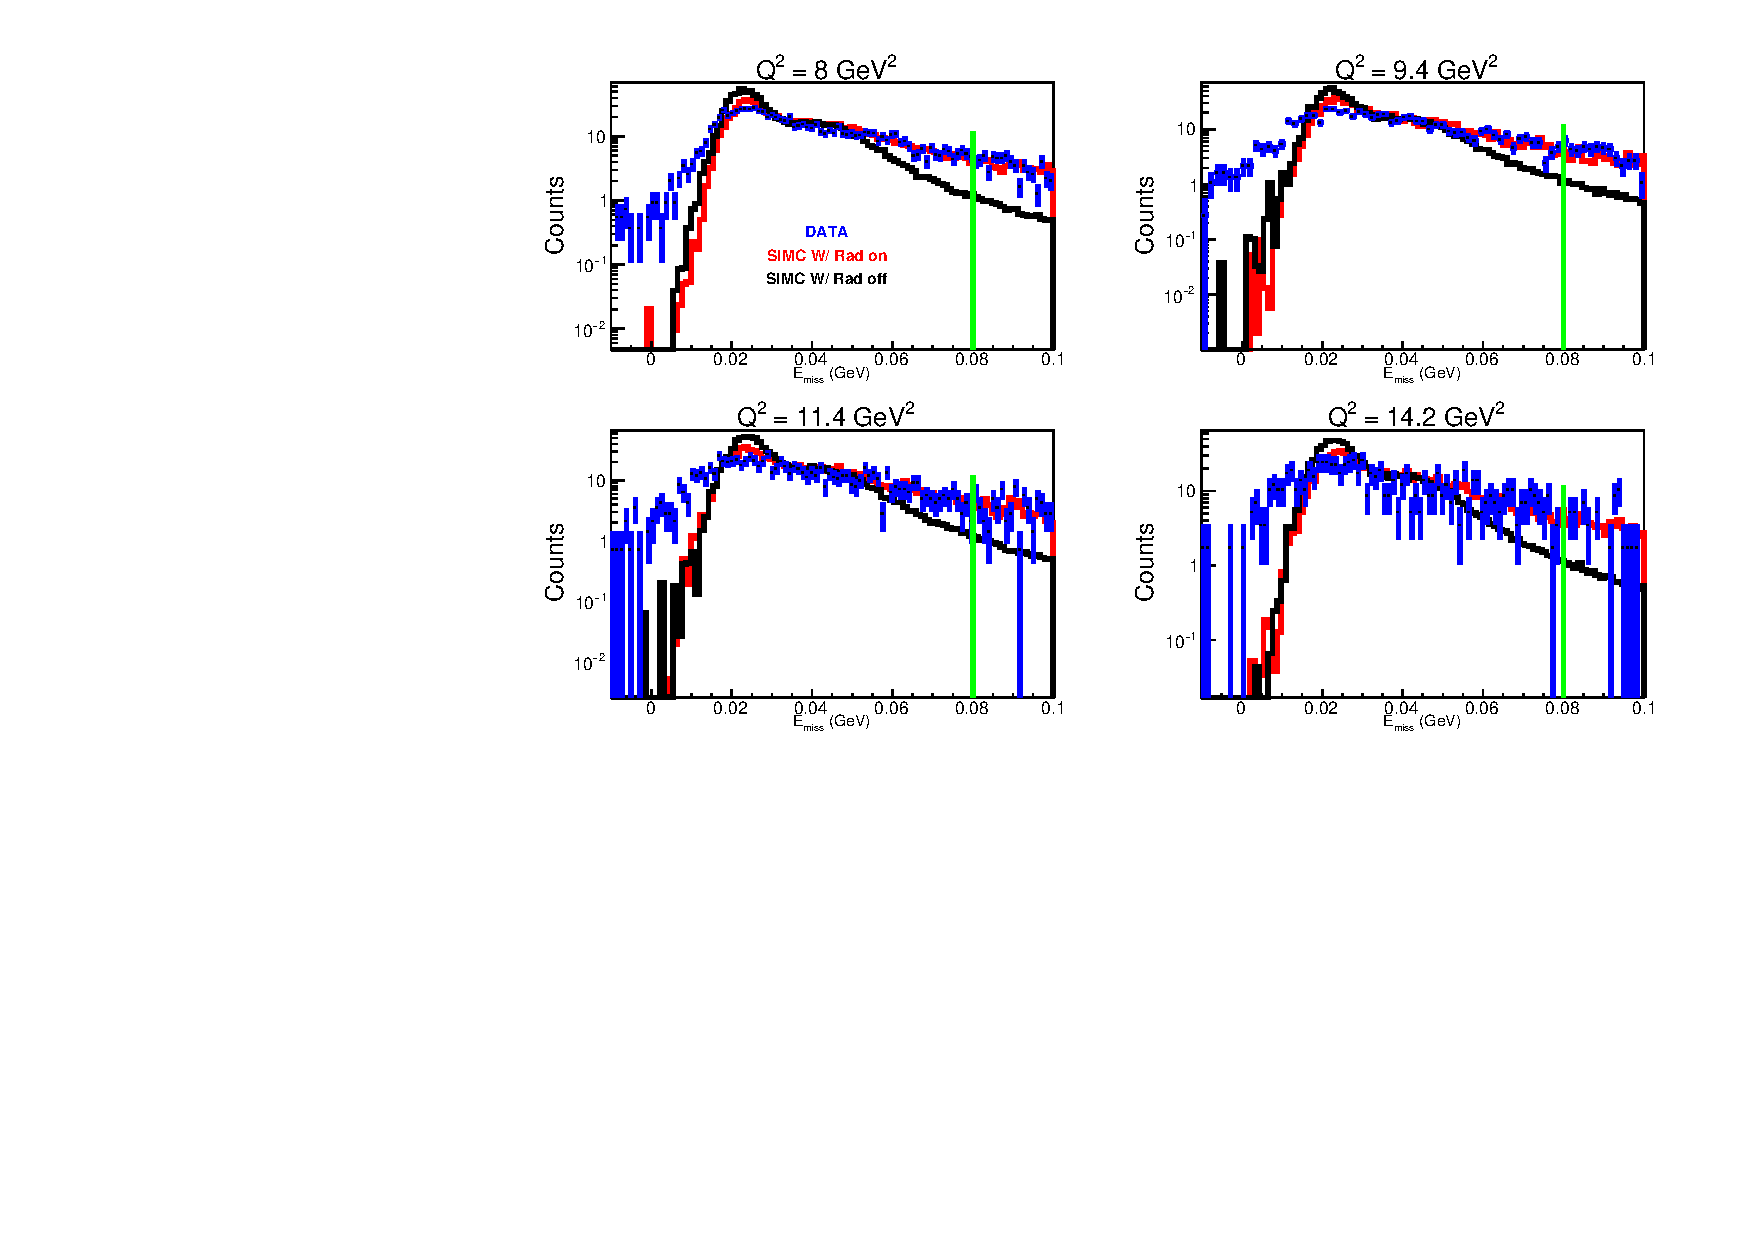
\includegraphics[width=1.0\textwidth]{chap5/Emiss_data_simc_w_and_wo_radcor.pdf}
    \caption{
            Distributions of missing energy $E_m$ measured in experiment (blue)
            and
            from Monte Carlo with (red) and without (black) radiative
            corrections.
            Data are for ${}^{12}C(e,e'p)$.
            }
    \label{fig:Emiss_data_simc_w_and_wo_radcor}
\end{figure}


